\section{"4" Верификация преобразователя силы}

\begin{frame}[t]{Верификация преобразователя силы}
\framesubtitle{}
\begin{columns}[T,onlytextwidth]
\begin{column}{0.69\textwidth}
    \small
    Охарактеризовать материал для случаев, когда площадь приложения силы меньше, чем площадь активной части сенсора.

    \textbf{Идея решения}: Разработка двух экспериментов: 
    
    1. Статический --- прикладывается статический груз с размером в сенсор для \underline{калибровки}.\\
    2. Динамический --- чувствительная область представляется в виде сетки $4\times4$. Происходит касание каждой области с одинаковым давлением, но разной площадью контакта.

    \textbf{Входные данные}: показания разработанного датчика и значение реально приложенной нагрузки.

    \textbf{Выходные данные}: разница между нормализованным значением с датчика и реальной нагрузкой.

    \textbf{Допустимая ошибка}: 10\%

    \textbf{Предположения}: 1) материал обладает вязко-эластичными свойствами, поэтому надо учитывать гистерезис.
\end{column}
\begin{column}{0.29\textwidth}
    \vspace{-1.0cm}
\begin{figure}[H]
\begin{subfigure}{0.99\textwidth}
        \centering
        \centering\includegraphics[height=3cm,width=1\textwidth,keepaspectratio,page=5]{./tikz_pictures.pdf}
        \caption*{Поверхность \\ как $4\times4$ сетка}
\end{subfigure}

\begin{subfigure}{0.99\textwidth}
    \centering\includegraphics[height=3cm,width=1\textwidth,keepaspectratio,page=4]{./tikz_pictures.pdf}
    \caption*{Все насадки}
\end{subfigure}

\end{figure}
\end{column}
\end{columns}
\end{frame}

\note{Имея конструкцию ноги, возможно разработать сенсор, подходящий для конкретной задачи. Как было сказано ранее, необходимо охарактеризовать материал для случаев когда площадь приложения силы меньше, чем площадь активной части сенсора.

Для этого было разработано 2 эксперимента. Первый, статический, где на объект прикладывался статический груз с разрмером сенсора, нужен для калибровки. Таким образом я считал, что все сенсоры работают единообразно.

Второй, динамический, основной. Для этого сенсор представлялся в виде сетки 4х4, на картинке. С помощью эталонного датчика силы, на который была прикреплена насадка, обеспечивающую конкретную площадь контакта, проводилась касание каждой области сетки.

Потом нормализовались значения между эталонным датчиком (он принимался за 1, и откалиброванным исследуемым датчиком и смотрелась разница. Допустимой ошибкой я посчитал 10 процентов.
}

\begin{frame}[t]{Статический эксперимент}
    \begin{columns}[T,onlytextwidth]
        \begin{column}{0.52\textwidth}
            \begin{eqnarray*}
                V_{out} = V_0 + p[k_p + k_e(1-e^\frac{-(t-t_0)}{\tau_{res}})](1-e^{-\frac{A}{p}}) \\
                k_p = A_1e^{-A_2p}; \tau_{res} = B_0 + B_1e^{-\frac{p}{B_2}}
            \end{eqnarray*}
            Где $V_0$ -- начальное напряжение, \\ $p$ -- приложенное давление, \\ $A_i,\ B_i,\ \tau_{res},\ k_i$ искомые параметры, \\  $t$ -- текущее время, $t_0$ -- время начала нажатия.
            \\ \alert{Апробированна модель для калибровки датчика}
        \end{column}
        \begin{column}{0.45\textwidth}
            \begin{figure}[H]
                \begin{subfigure}{0.99\textwidth}
                    \centering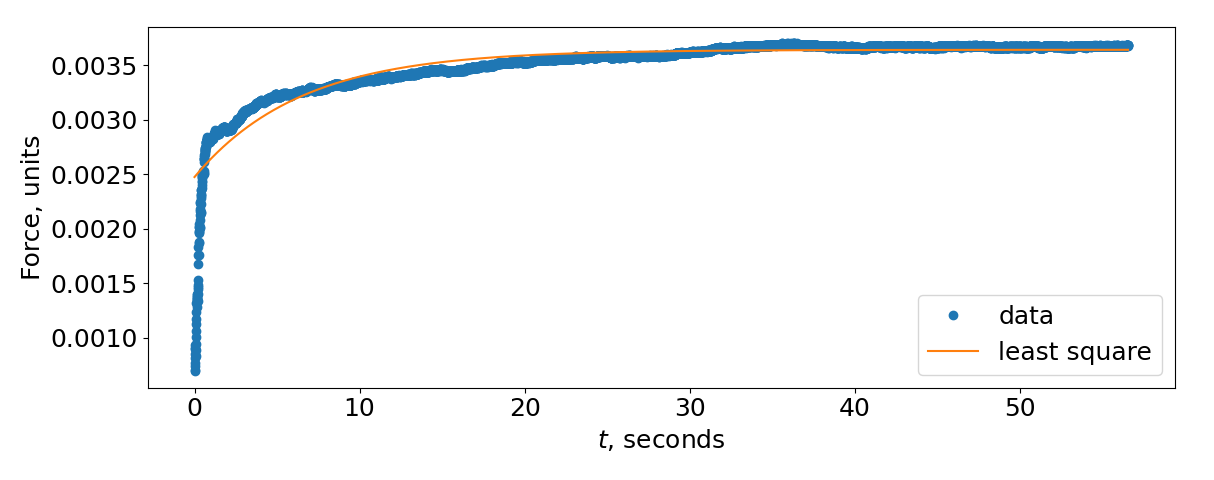
\includegraphics[height=2.8cm,width=1\textwidth,keepaspectratio]{least_square_model.png}
                \end{subfigure}
                \vspace{-1cm}

                \begin{subfigure}{0.99\textwidth}
                    \centering
                    \centering\includegraphics[height=3.4cm,width=1\textwidth,keepaspectratio,page=6]{./tikz_pictures.pdf}
                \end{subfigure}
            \end{figure}
        \end{column}
    \end{columns}
\end{frame}

\note{Статический эксперимент. Для калибровки использовался робастный метод наименьших квадратов, экспериментальная установка справа, формула для регрессии - слева. Она основана на знании того, что у нас вязко-эластичный материал, обладающий гистерезисом. Поэтому необходимо учитывать время контакта с поверхностью.

Как можно заметить по графику справа, эта формула подходит для калибровки.}

\begin{frame}[t]{Динамический эксперимент: установка}
    \begin{columns}[T,onlytextwidth]
        \begin{column}{0.39\textwidth}
            \begin{itemize}
                \item Управление силой нажатия {\\ \alert{Импедансное управления}}
                \item Повторяемость эксперимента по силе и позиции{\\ \alert{Добавив манипулятор и камеру}}
                \item Возможность нажимать только на часть сенсора{\\ \alert{Насадки для манипулятора}}
            \end{itemize}
        \end{column}
        \begin{column}{0.8\textwidth}
            \scalebox{0.81}{
                \centering\includegraphics[height=6cm,width=1\textwidth,keepaspectratio,page=7]{./tikz_pictures.pdf}
            }
        \end{column}
    \end{columns}
\end{frame}

\note{Так как динамический эксперимент требует многократное повторение действий, где важна точность силы нажатия, то было решено создать автоматизированную робототехническую установку. Управление силой нажатия было реализовано с помощью импедансного управления. Минимизация ошибки установки было реализовано с помощью технического зрения.
}

\begin{frame}[t]{Результаты динамического эксперимента}
    \begin{figure}[H]
        \begin{subfigure}{0.49\textwidth}
            \centering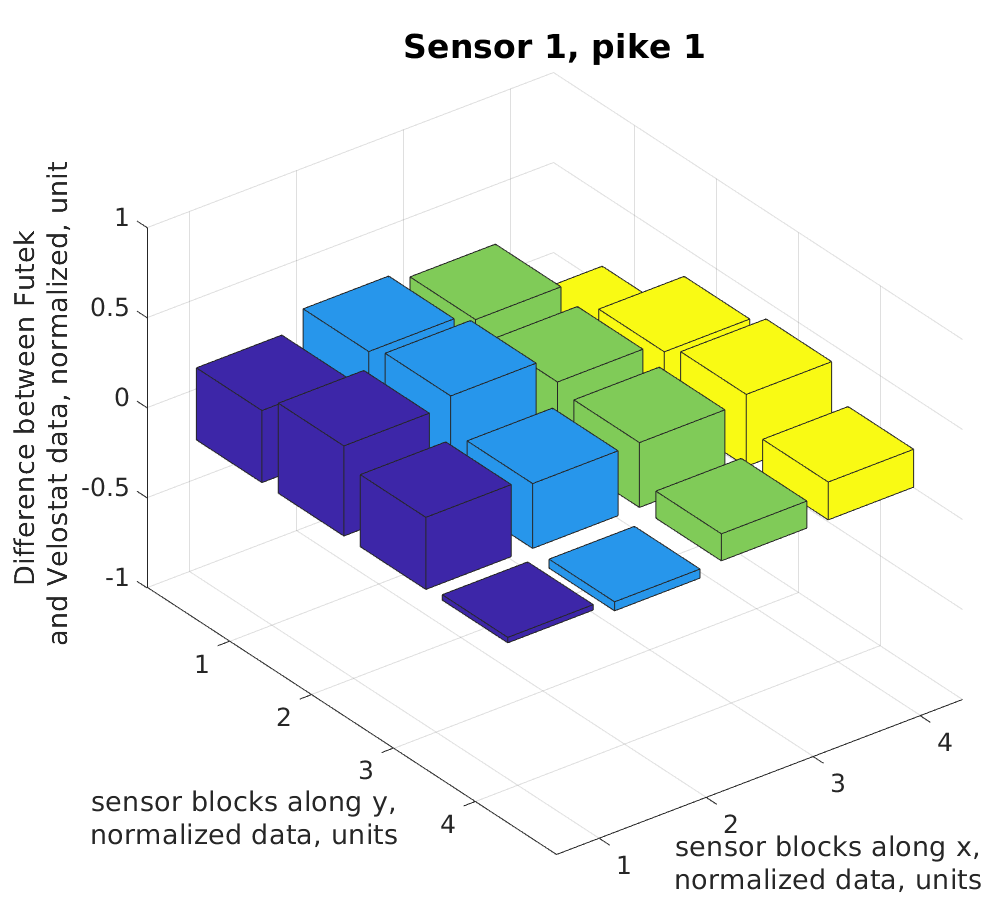
\includegraphics[height=5cm,width=1\textwidth,keepaspectratio]{sens1_pike1.png}
            \caption*{2 мм диаметр насадки}
        \end{subfigure}
        \begin{subfigure}{0.49\textwidth}
            \centering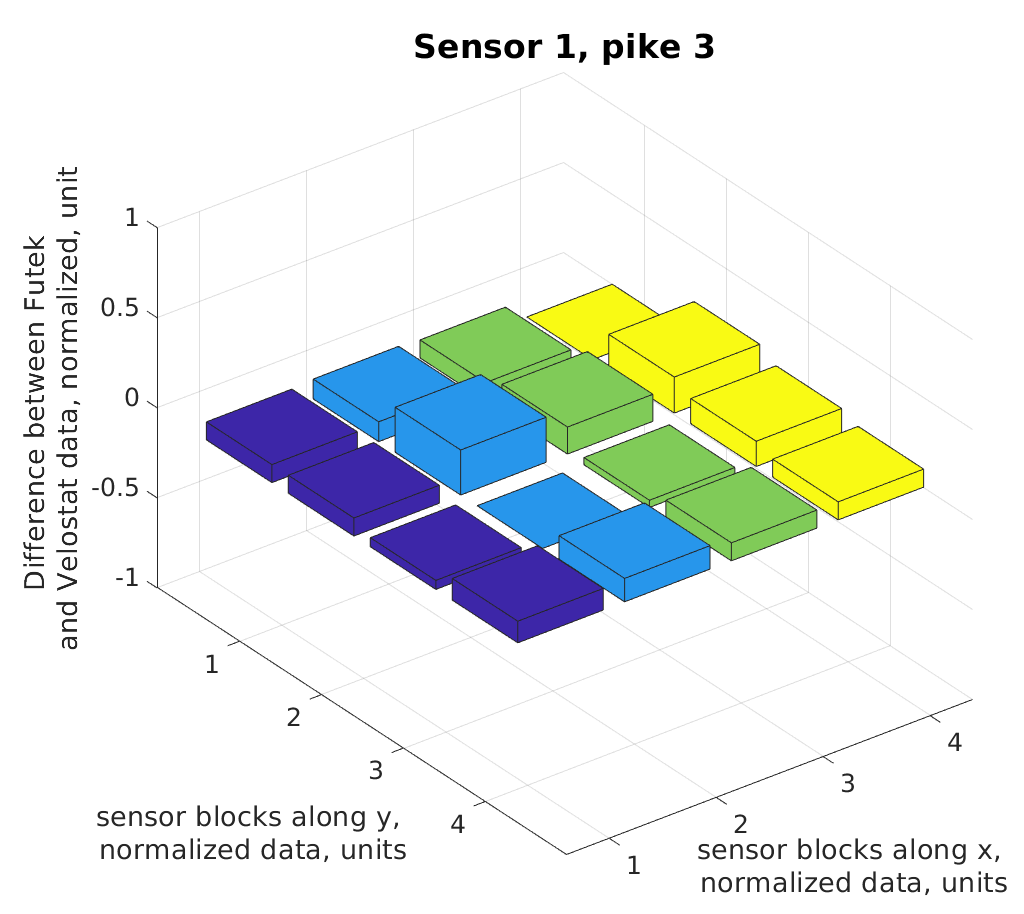
\includegraphics[height=5cm,width=1\textwidth,keepaspectratio]{sens1_pike3.png}
            \caption*{8 мм диаметр насадки}
        \end{subfigure}
    \end{figure}
    \vspace{-0.8cm}
    \alert{Одинаковые данные, когда площадь нажатия превышает 25\% от площади датчика}
\end{frame}

\note{Результатом изысканий получилось, что можно использовать сенсор, когда площадь нажатия превышает 25 площади датчика.

На слайде можно увидеть 3д гистограмму, где представлена нормализованная разница между эталонным датчиком и исследуемым. Слева при использования насадки в 2 мм диаметром, а справа при 8 мм.
}